\documentclass{article}

\usepackage{microtype}
\usepackage{graphicx}
\usepackage{subfigure}
\usepackage{booktabs}
\usepackage{hyperref}
\usepackage{amsfonts}
\usepackage{amsmath}

\newcommand{\theHalgorithm}{\arabic{algorithm}}
\usepackage[accepted]{icml2019}

% If accepted, instead use the following line for the camera-ready submission:
%\usepackage[accepted]{icml2018}

% The \icmltitle you define below is probably too long as a header.
% Therefore, a short form for the running title is supplied here:
\icmltitlerunning{Action Grammars: A Grammar Induction-Based Method for
           Learning Temporally Extended Actions}

\begin{document}

\twocolumn[
\icmltitle{Action Grammars: A Grammar Induction-Based Method for \\
           Learning Temporally Extended Actions}

% It is OKAY to include author information, even for blind
% submissions: the style file will automatically remove it for you
% unless you've provided the [accepted] option to the icml2018
% package.

% List of affiliations: The first argument should be a (short)
% identifier you will use later to specify author affiliations
% Academic affiliations should list Department, University, City, Region, Country
% Industry affiliations should list Company, City, Region, Country

% You can specify symbols, otherwise they are numbered in order.
% Ideally, you should not use this facility. Affiliations will be numbered
% in order of appearance and this is the preferred way.
\icmlsetsymbol{equal}{*}

\begin{icmlauthorlist}
\icmlauthor{Robert Tjarko Lange}{ecn}
\icmlauthor{Aldo Faisal}{icl}
\end{icmlauthorlist}

\icmlaffiliation{icl}{Department of Computing, Imperial College London, London, United Kingdom}
\icmlaffiliation{ecn}{Einstein Center for Neurosciences Berlin, Berlin, Germany}

\icmlcorrespondingauthor{Robert Tjarko Lange}{robert.lange17@ic.ac.uk}

% You may provide any keywords that you
% find helpful for describing your paper; these are used to populate
% the "keywords" metadata in the PDF but will not be shown in the document
\icmlkeywords{Machine Learning, ICML}

\vskip 0.3in
]

%\printAffiliationsAndNotice{}  % leave blank if no need to mention equal contribution
\printAffiliationsAndNotice{\icmlEqualContribution} % otherwise use the standard text.

\begin{abstract}
Temporal abstraction allows efficient re-usability of sequential behavior across the state space. Learning semantically meaningful macro-actions defines a key challenge of Hierarchical Reinforcement Learning. Here, we introduce a fully end-to-end algorithmic framework which builds a grammatical memory buffer. By treating an agent's trace as a sentence sampled from the policy-conditioned environment, the agents learns hierarchical sub-structures using powerful unsupervised grammatical inference algorithms.  
\end{abstract}

\section{Introduction}\label{ch1:intro}
Goal-driven behavior is inherently driven by the hierarchical nature of the imposed task. Hierarchical Reinforcement Learning (HRL) intends to solve the credit assignment problem of the agent by modeling different time-scales of decision making. 

\begin{figure}[H]
    \centering
    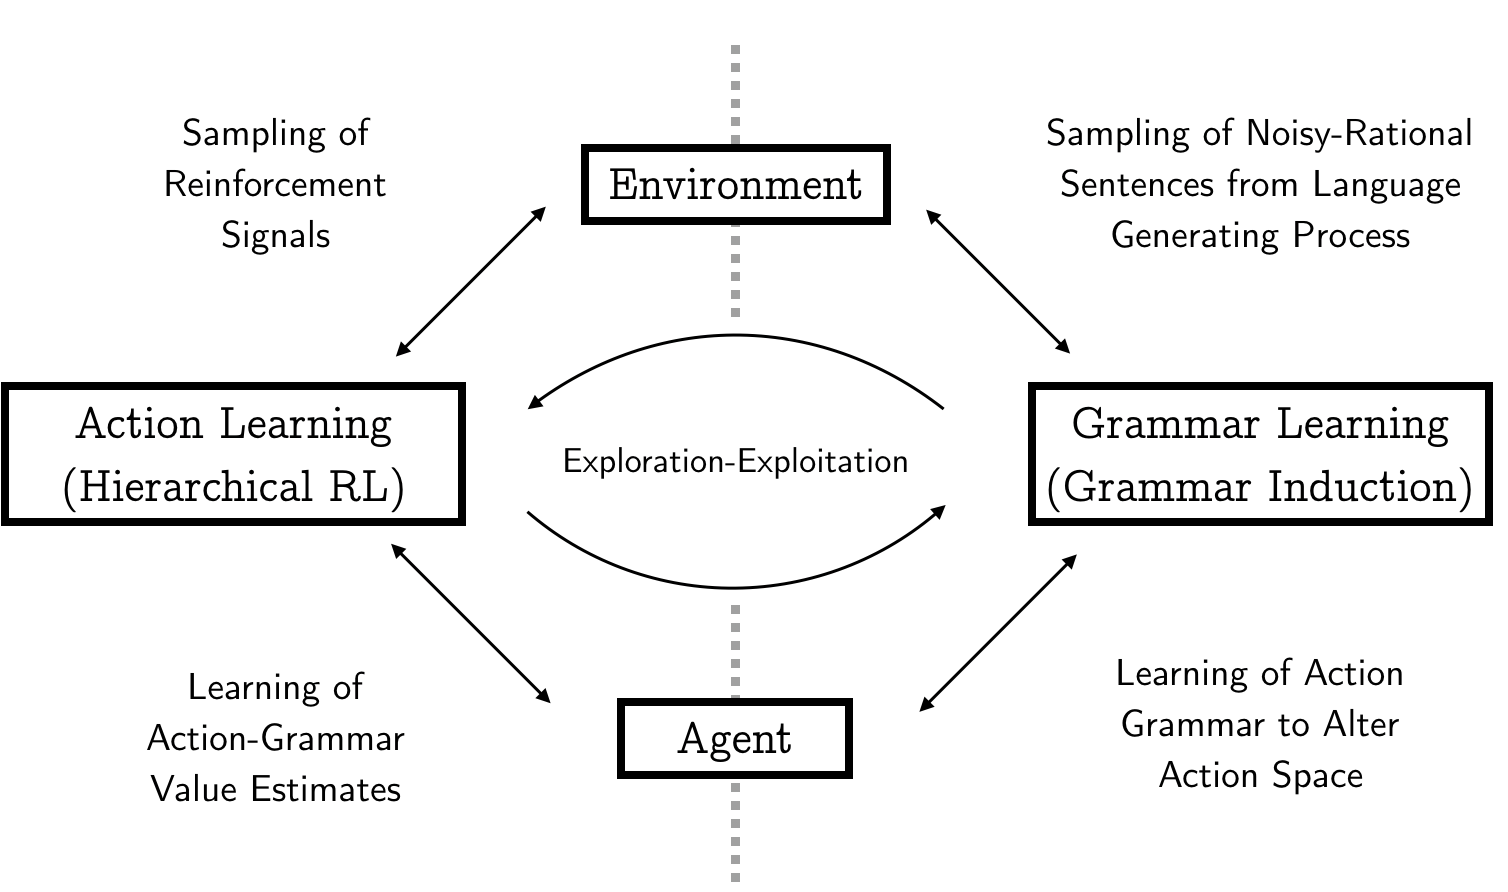
\includegraphics[width=\linewidth]{figures/concept_al_gl.png}
    \caption{Action Grammars for HRL}
    \label{fig:loop_ag}
\end{figure}

\newpage
\section{Related Work}

\newpage
\section{Technical Background}

\subsection{Temporally-Extended Actions}

Semi-Markov Decision Processes extend the classical MDP setting to incorporate not only environmental uncertainty but also time uncertainty. Instead of dealing with a Dirac waiting distribution, the time between individual decisions is modeled as a random variable, $\tau \in \mathbb{Z}_{++}$. It is described by the probability distribution $P(s', \tau| s, m)$  which characterizes the the joint likelihood of transitioning from state $s \in \mathcal{S}$ into state $s'$ in $\tau$ time steps given action $m$ was pursued.

Thereby, SMDPs allow one to elegantly model the execution of actions which extend over multiple time-steps (e.g. sequences of primitive actions or sub-policy execution). Multiple different hierarchical action structures have been proposed. In this work we focus on the most simplest, namely macro-actions. Simply put, macro-actions specify the sequential and deterministic execution of multiple primitive actions.  

\subsection{Context-Free Grammars}


\newpage
\section{Context-Free Action Grammars}

\begin{figure}[H]
    \centering
    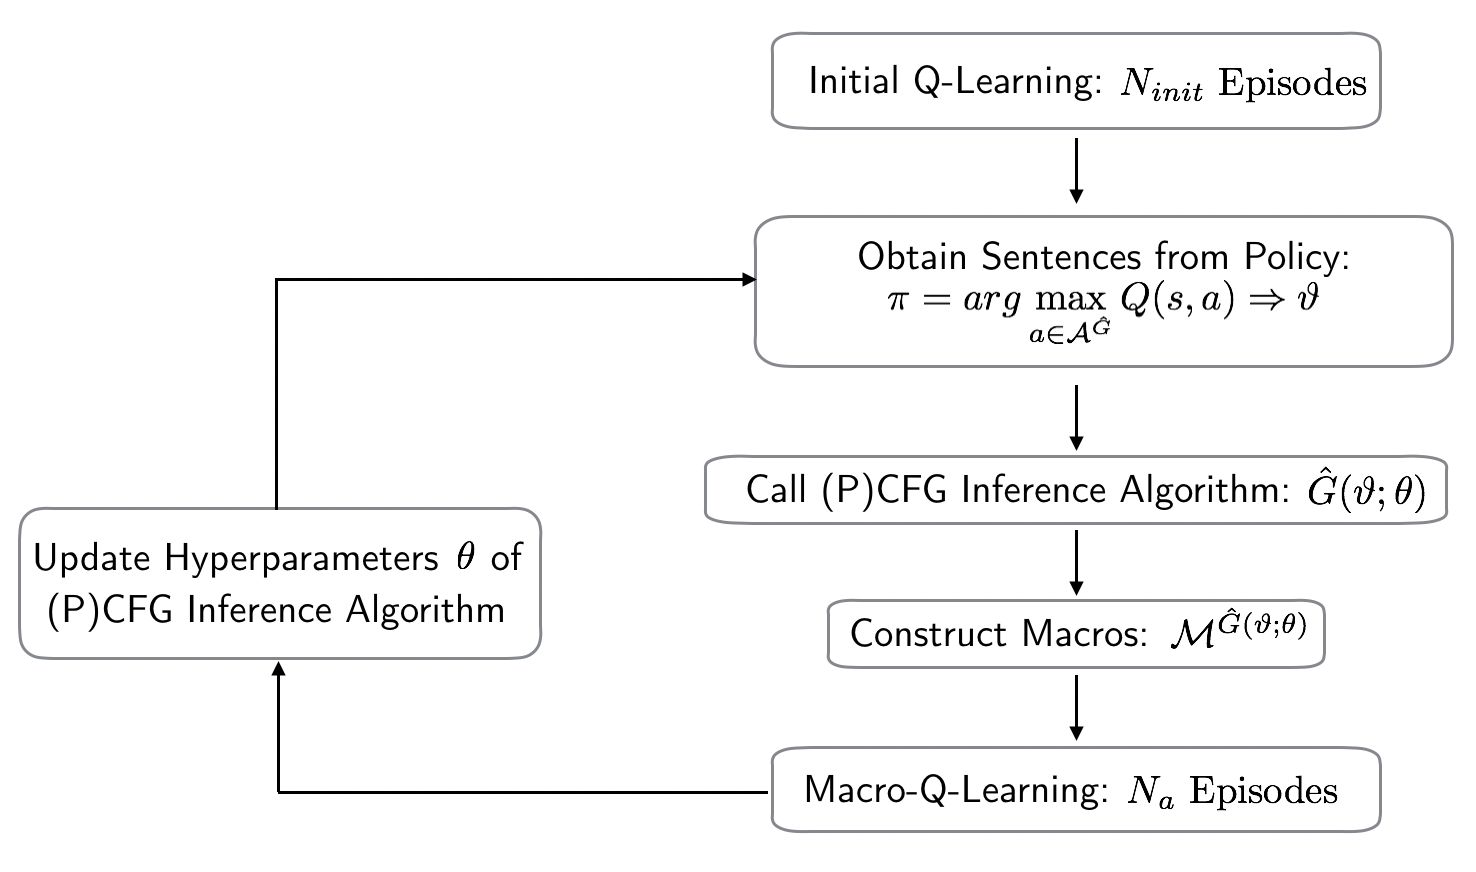
\includegraphics[width=0.495\textwidth]{figures/concept_online_macro_learning.png}
    \caption{Action Grammars: A General Pipeline}
    \label{fig:my_label}
\end{figure}

\begin{align*}
    L(\theta) := &\mathbb{E}_{s,m,r^{\tau_m},s', \tau \sim D_{\tau_m}} [(r^{\tau_m} + \\ & \gamma^{\tau_m} \max_{m'} Q(s',m';\theta^-) - Q(s,m; \theta))^2]
\end{align*}


\newpage
\section{Experiments}

\subsection{Towers of Hanoi}

\begin{figure}[H]
    \centering
    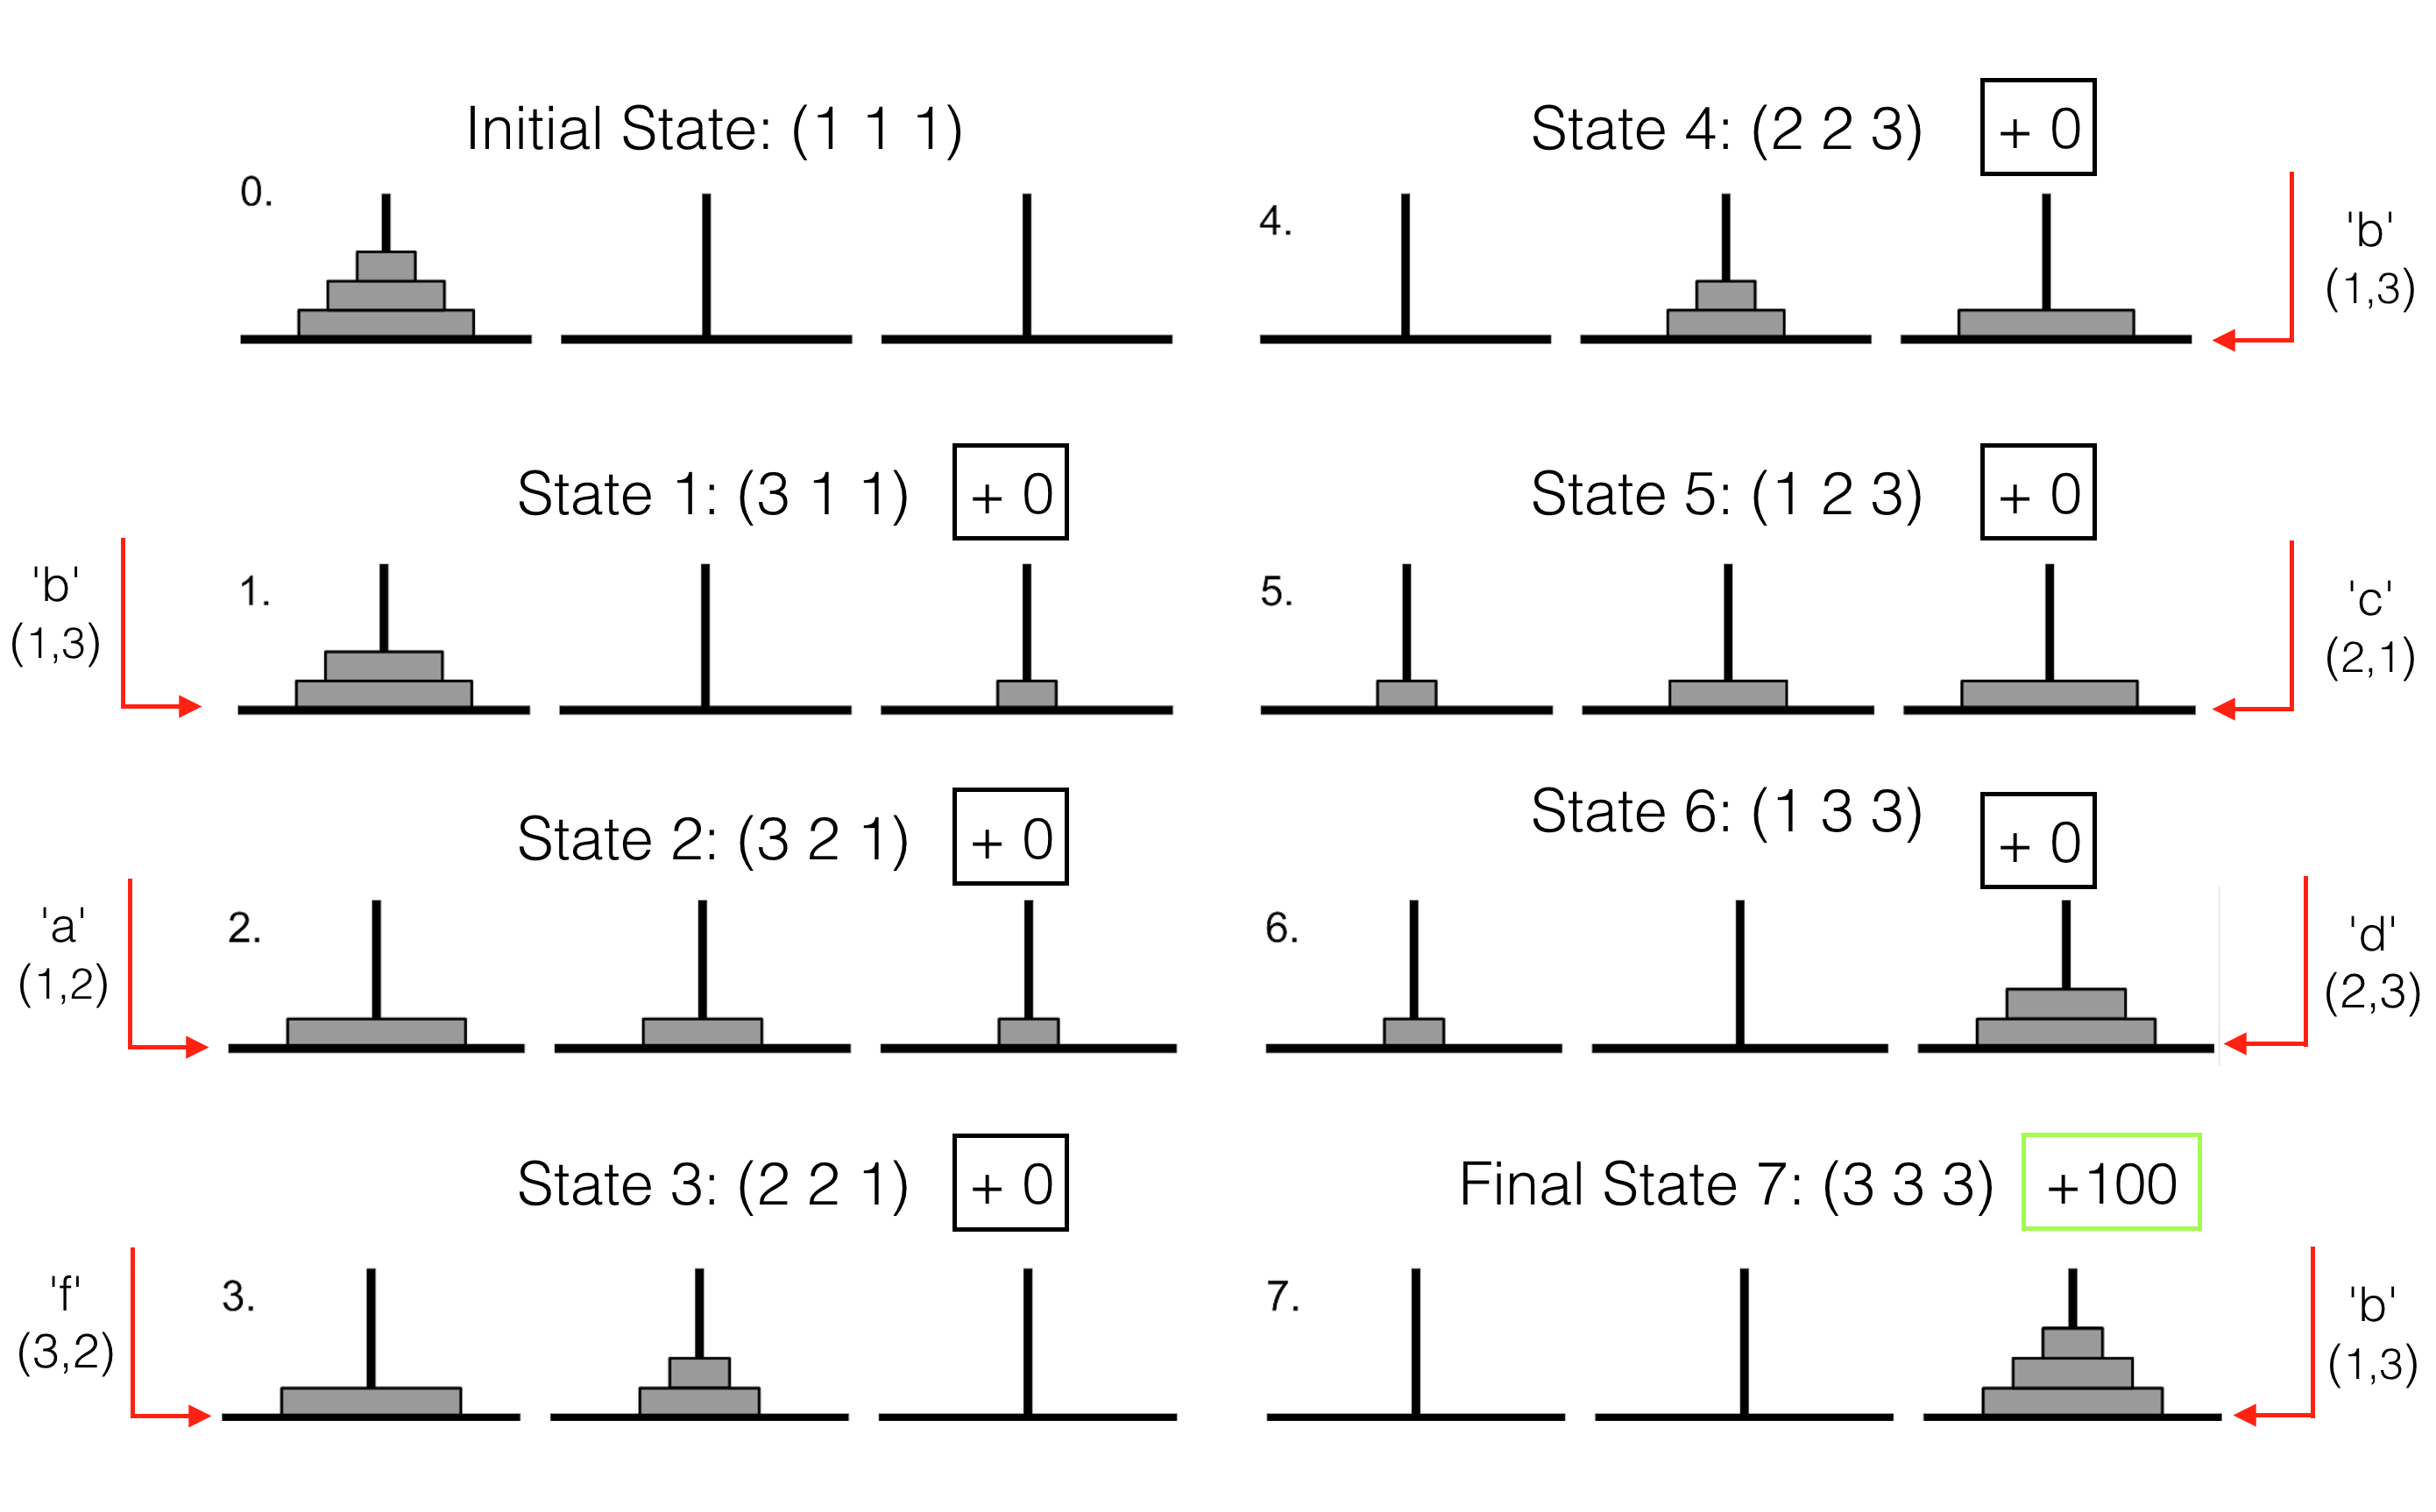
\includegraphics[width=0.45\textwidth]{figures/hanoi_problem.png}
    \caption{Optimal Solution for Towers of Hanoi Environment for 3 disks ($N=3$)}
    \label{fig:my_label}
\end{figure}

Visualize the grammar learned

\subsection{ATARI Environments}

\newpage
\section{Discussion}

This work has introduced a computational framework which connects the field of context-free grammar inference with Hierarchical Reinforcement Learning. Going forwards, we interested in extending this approach to both options as well as probabilistic grammars. One potential way of achieving this might be by defining a probabilistic termination condition with the help of syntactic surprise\citep{Hale_2003, Hale_2006}. Furthermore, building a grammatical dictionary might be promising for efforts in continual or life-long learning.

\begin{algorithm}[H]
   \caption{Bubble Sort}
   \label{alg:example}
\begin{algorithmic}
   \STATE {\bfseries Input:} data $x_i$, size $m$
   \REPEAT
   \STATE Initialize $noChange = true$.
   \FOR{$i=1$ {\bfseries to} $m-1$}
   \IF{$x_i > x_{i+1}$}
   \STATE Swap $x_i$ and $x_{i+1}$
   \STATE $noChange = false$
   \ENDIF
   \ENDFOR
   \UNTIL{$noChange$ is $true$}
\end{algorithmic}
\end{algorithm}


\newpage
\bibliography{HRL}
\bibliographystyle{icml2018}

\end{document}